\begin{savequote}[45mm]
\ascii{Any fool can write code that a computer can understand. Good programmers write code that humans can understand.}
\qauthor{\ascii{- Martin Flower}}
\end{savequote}

\chapter{破冰之旅} 
\label{ch:bazel-tour}

\section{安装}

\begin{content}

本例以\ascii{Ubuntu 18.04}为例,讲述\ascii{Bazel}的安装方式。

\subsection{二进制安装}

首先,安装\ascii{Bazel}所依赖包。

\begin{nodiff}{安装依赖}
 \begin{python}
$ sudo apt-get install pkg-config zip g++ zlib1g-dev unzip python
 \end{python}
\end{nodiff}

从\ascii{Github}上下载\ascii{Bazel}最新的版本,此处以版本\ascii{0.23.0}为例。

\begin{nodiff}{下载安装包}
 \begin{python}
$ bazel_version=0.23.0
$ bazel_binary=https://github.com/bazelbuild/bazel/releases/download/
$ bazel_binary+=$bazel_version/bazel-$bazel_version-installer-linux-x86_64.sh
$ wget -c $bazel_binary
 \end{python}
\end{nodiff}

修改脚本的权限,运行脚本启动安装过程。使用\ascii{--user}选项,\ascii{Bazel}将安装到\ascii{~/home/bin}目录。

\begin{nodiff}{安装Bazel}
 \begin{python}
$ chmod +x bazel-$bazel_version-installer-linux-x86_64.sh
$ ./bazel-$bazel_version-installer-linux-x86_64.sh --user
 \end{python}
\end{nodiff}

添加\ascii{~/home/bin}目录至环境变量\ascii{PATH}之中。

\begin{nodiff}{添加PATH}
 \begin{python}
$ echo 'export PATH=$PATH:$HOME/bin' >> ~/.bashrc
$ source ~/.bashrc
 \end{python}
\end{nodiff}

最后,通过执行如下命令验证安装是否成功。

\begin{nodiff}{验证}
 \begin{python}
$ bazel version
 \end{python}
\end{nodiff}

\subsection{APT安装}

在\ascii{Ubutu}中,也可以使用\ascii{apt}安装\ascii{Bazel}。因为\ascii{Bazel}主要使用\ascii{Java}实现,因此需要实现安装\ascii{JVM}。

\begin{nodiff}{安装依赖}
 \begin{python}
$ sudo apt-get install openjdk-8-jdk
 \end{python}
\end{nodiff}

在系统添加\ascii{Bazel}的软件源。

\begin{nodiff}{Bazel源}
 \begin{python}
$ cat <<EOF | sudo tee /etc/apt/sources.list.d/bazel.list
deb [arch=amd64] http://storage.googleapis.com/bazel-apt stable jdk1.8
EOF
$ curl https://bazel.build/bazel-release.pub.gpg | sudo apt-key add -
 \end{python}
\end{nodiff}

执行如下命令,安装\ascii{Bazel}。

\begin{nodiff}{安装Bazel}
 \begin{python}
$ sudo apt-get update
$ sudo apt-get install bazel
 \end{python}
\end{nodiff}

\end{content}

\section{入门}

\begin{content}

\subsection{C++工程}

新建一个\ascii{C++}工程,物理组织如\refig{bazel-tour-hello-world-tree}所示。它包括\ascii{lib}和\ascii{main}两个包。\ascii{WORKSPACE}为空文件,表示该项目不依赖于第三方库,仅依赖标准库。

\begin{figure}[H]
\centering
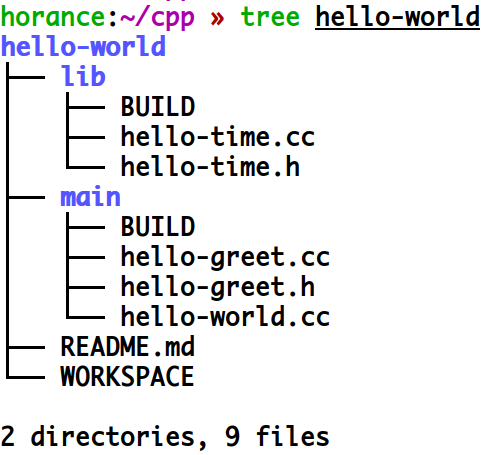
\includegraphics[width=0.5\textwidth]{figures/bazel-tour-hello-world-tree.png}
\caption{工程组织} 
 \label{fig:bazel-tour-hello-world-tree}
\end{figure}

\subsubsection{lib包}

在\ascii{lib}包中,包含\ascii{hello-time.h, hello-time.cc}两个源文件。

\begin{nodiff}{lib/hello-time.h}
 \begin{c++}
#ifndef LIB_HELLO_TIME_H_      
#define LIB_HELLO_TIME_H_

void print_localtime();

#endif
 \end{c++}
\end{nodiff}

\begin{nodiff}{lib/hello-time.cc}
 \begin{c++}
#include "lib/hello-time.h"
#include <ctime>         
#include <iostream>

void print_localtime() {
  std::time_t result = std::time(nullptr);
  std::cout << std::asctime(std::localtime(&result));
}
 \end{c++}
\end{nodiff}

在规则\ascii{//lib:hello-time}定义之中,声明了\ascii{visibility}属性,\ascii{//main:\_\_pkg\_\_}表示该规则对\ascii{main}包可见。

\begin{nodiff}{lib/BUILD}
 \begin{python}
cc_library(
    name = "hello-time", 
    srcs = ["hello-time.cc"], 
    hdrs = ["hello-time.h"],  
    visibility = ["//main:__pkg__"],
)
 \end{python}
\end{nodiff}

\subsubsection{main包}

在\ascii{main}包中,定义了一个规则\ascii{//main:hello-greet},它实现了\ascii{get\_greet}函数。

\begin{nodiff}{main/hello-greet.h}
 \begin{c++}
#ifndef MAIN_HELLO_GREET_H_
#define MAIN_HELLO_GREET_H_

#include <string>

std::string get_greet(const std::string &thing);
      
#endif
 \end{c++}
\end{nodiff}

\begin{nodiff}{main/hello-greet.cc}
 \begin{c++}
#include "main/hello-greet.h"             
#include <string>

std::string get_greet(const std::string& who) {
  return "Hello " + who;
}
 \end{c++}
\end{nodiff}

在\ascii{main}包中,还定义了另一个规则\ascii{//main:hello-world},它实现了\ascii{main}函数。

\begin{nodiff}{main/main.cc}
 \begin{c++}
#include "lib/hello-time.h"
#include "main/hello-greet.h"
#include <iostream>

int main(int argc, char** argv) {
  std::cout << get_greet("world") << std::endl;
  print_localtime();
  return 0;
}
 \end{c++}
\end{nodiff}

重点关注一下规则\ascii{//main:hello-world}的\ascii{deps}属性,因为\ascii{//main:hello-world}和\ascii{//main:hello-greet}在同一个包中,可简写为\ascii{:hello-greet};但是,\ascii{//main:hello-world}和\ascii{//main:hello-time}不在同一个包中,因此需要完整的路径。


\begin{nodiff}{main/BUILD}
 \begin{python}
cc_library(            
    name = "hello-greet",
    srcs = ["hello-greet.cc"],
    hdrs = ["hello-greet.h"], 
) 

cc_binary(
    name = "hello-world",
    srcs = ["hello-world.cc"],
    deps = [             
        ":hello-greet",
        "//lib:hello-time",       
    ],
)
 \end{python}
\end{nodiff}

执行如下命令,构建目标\ascii{//main:hello-world}。

\begin{nodiff}{构建}
 \begin{python}
$ bazel build //main:hello-world
 \end{python}
\end{nodiff}

构建成功后,生成可执行程序\ascii{bazel-bin/main/hello-world}。

\begin{nodiff}{执行}
 \begin{python}
$ bazel-bin/main/hello-world
Hello world
Wed Feb 27 10:49:05 2019
 \end{python}
\end{nodiff}

\subsection{解析依赖}

执行如下命令,可以得到以\ascii{//main:hello-world}为根节点的\ascii{DAG}图,如\refig{bazel-tour-hello-world-deps}所示。

\begin{nodiff}{构建图}
 \begin{python}
$ xdot <(bazel query --nohost_deps --noimplicit_deps 'deps(//main:hello-world)' --output graph)
 \end{python}
\end{nodiff}

\begin{figure}[H]
\centering
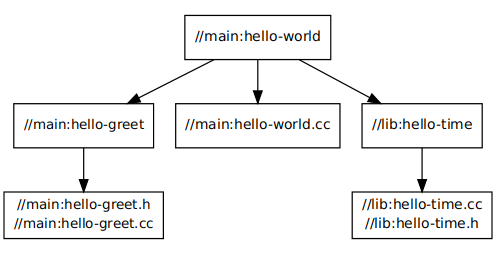
\includegraphics[width=0.8\textwidth]{figures/bazel-tour-hello-world-deps.png}
\caption{依赖图: //main:hello_world} 
 \label{fig:bazel-tour-hello-world-deps}
\end{figure}

\end{content}
